\documentclass[../main.tex]{subfiles}
\begin{document}
\section{Validation}
The generalization performance of a learning method relates to its predic- tion capability on independent test data. Assessment of this performance is extremely important in practice, since it guides the choice of learning method or model, and gives us a measure of the quality of the ultimately chosen model.
In this chapter we describe and illustrate the key methods for performance assessment, and show how they are used to select models. 

\subsection{Motivation (Mitchell)}
In many cases it is important to evaluate the performance of learned hypotheses as precisely as possible. One reason is simply to understand whether to use the hypothesis. For instance, when learning from a limited-size database indicating the effectiveness of different medical treatments, it is important to understand as precisely as possible the accuracy of the learned hypotheses. A second reason is that evaluating hypotheses is an integral component of many learning methods.\\
Estimating the accuracy of a hypothesis is relatively straightforward when data is plentiful. However, when we must learn a hypothesis and estimate its future accuracy given only a limited set of data, two key difficulties arise:

\begin{itemize}
    \item \textbf{Bias in the estimate}. First, the observed accuracy of the learned hypothesis over the training examples is often a poor estimator of its accuracy over future examples. Because the learned hypothesis was derived from these examples, they will typically provide an optimistically biased estimate of hypothesis accuracy over future examples. This is especially likely when the learner considers a very rich hypothesis space, enabling it to overfit the training examples. To obtain an unbiased estimate of future accuracy, we typically test the hypothesis on some set of test examples chosen independently of the training examples and the hypothesis.
    
    \item \textbf{Variance in the estimate}. Second, even if the hypothesis accuracy is mea- sured over an unbiased set of test examples independent of the training examples, the measured accuracy can still vary from the true accuracy, de- pending on the makeup of the particular set of test examples. The smaller the set of test examples, the greater the expected variance.
\end{itemize}

\subsection{A premise: Bias-Variance}
Bias-Variance decomposition provides an useful framework to understand the validation issue, showing how the estimation of a model performance is difficult
\begin{itemize}
    \item Considering also the role of different training set realizations
    \item Showing again the need of a trade-off between fitting capability (bias) and model flexibility (variance) in different way
\end{itemize}

\noindent \textbf{Under/Over-fitting in a Bias-Variance plot}
\begin{figure}[H]
    \centering
    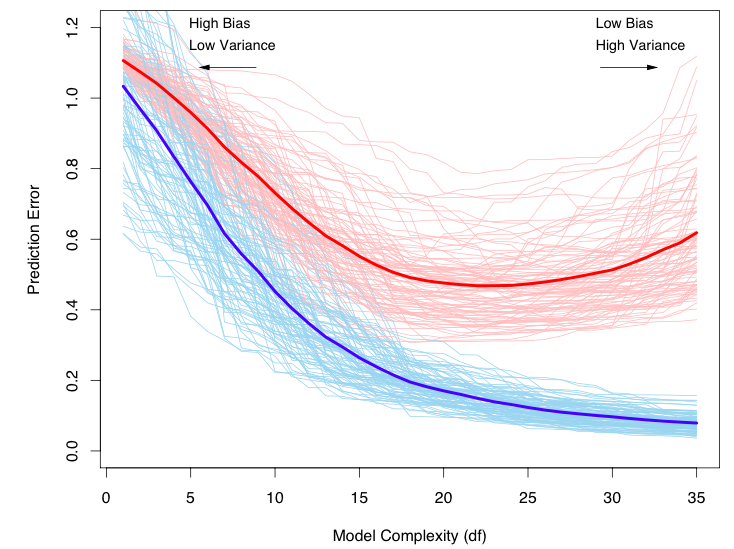
\includegraphics[scale = 0.4]{lectures/5_validation/5_bias_oufit_plot.png}
    \caption{Behavior of test sample and training sample error as the model complexity is varied. The light blue curves show the training error $\overline{err}$, while the light red curves show the conditional test error $Err_T$ for 100 training sets of size 50 each, as the model complexity is increased. The solid curves show the expected test error Err and the expected training error $E[\overline{err}]$.}
    \label{fig:5_bias_oufit_plot}
\end{figure}

In fig~\ref{fig:5_bias_oufit_plot} illustrates the important issue in assessing the ability of a learning method to generalize. Consider first the case of a quantitative or interval scale response. We have a target variable $Y$, a vector of inputs $X$, and a
prediction model $h(X)$ that has been estimated from a training set $T$.
The loss function for measuring errors between Y and f(X) is denoted by 
$L(Y,h(X))$ (E.g. mean (square) error).


Unfortunately training error is not a good estimate of the test error, as seen in Figure~\ref{fig:5_bias_oufit_plot}. Training error consistently decreases with model complexity, typically dropping to zero if we increase the model complexity enough. However, a model with zero training error is overfit to the training data and will typically generalize poorly.

\begin{itemize}
    \item we are looking for the best solution (minimal prediction – test error) searching a balancing between fitting (accuracy on training data) and model complexity
    
    \item Training set is not a good estimate of test error. Initially too many bias (under fitting, high TR error) than too high
    
    \item Assuming a tuning parameters $\theta$ (implicit or explicit) that varies the model complexity, we wish to find the value of $\theta$ that minimizes test error variance (low TR error but over fitting)
    
    \item Look for methods for estimating the expected error for a model
\end{itemize}

\noindent We can approximate the validation step:
\begin{itemize}
    \item \textbf{analytically}
    \begin{itemize}
        \item AIC, BIC (Akaike/Bayesian Information Criterion)
        \item MDL (Minimum Description Length) 
        \item SRM: Structural Risk Minimization and VC-dimension
    \end{itemize}
    
    \item \textbf{re-sampling}: efficient sample re-use 
    \begin{itemize}
        \item cross-validation: hold-out, K-fold CV, ...
        \item bootstrap
    \end{itemize}
\end{itemize}
In practice, often we can approximate the estimation on the data set by re-sampling.

\subsection{Model Selection and Assessment}
It is important to note that there are in fact two separate goals that we might have in mind:
\begin{itemize}
    \item \textbf{Model selection}: estimating the performance of
different learning models in order to choose the best one (to generalize)
– this includes search the best hyper-parameters of your model (e.g. polynomial order, number of units in a NN, lambda, eta, ... ...).
\begin{center}
    \textbf{It returns a model}
\end{center}
\item \textbf{Model assessment}: having chosen a final model (or a class of models), estimating/evaluating its prediction error/ risk (generalization error) on new test data (measure of the quality of the ultimately chosen model)
\begin{center}
    \textbf{It returns an estimation value}
\end{center}
\end{itemize}
So, usually the dataset is divided in three disjoint sets: a training set, a validation set, and a test set.
\begin{figure}[H]
    \centering
    
\includegraphics[scale  =0.4]{lectures/5_validation/5_data_partition_for_validation.png}
\end{figure}
The \textbf{training set} is used to fit the models; \textbf{the validation set} (or selection set) is used to estimate prediction error for model selection and can be used to select the best models (e.g. hyper-parameters tuning); 
\begin{center}
    TR+VL sometimes are joitnly called development/design set\\ i.e. used to build the final model
\end{center}
The \textbf{test set} is used for assessment of the generalization error of the final chosen model. The test set should be kept in a “vault,” and be brought out only at the end of the data analysis.\\

Suppose instead that we use the test-set repeatedly, what if test set is used in a (repeated) design cycle and choosing the model with smallest test-set error?
\begin{itemize}
    \item We are making model selection and not reliable assessment (estimation of expected generalization error) and we need a new test set for the generalization error.

    \item In that case, used test set error provide an overoptimistic evaluation of the true test error ($\rightarrow$ we will see how easy is to obtain very high classification accuracy over random task even using the test set only implicitly)
\end{itemize}

\textbf{TR/VL/TS by a simple schema}
\begin{figure}[H]
    \centering
    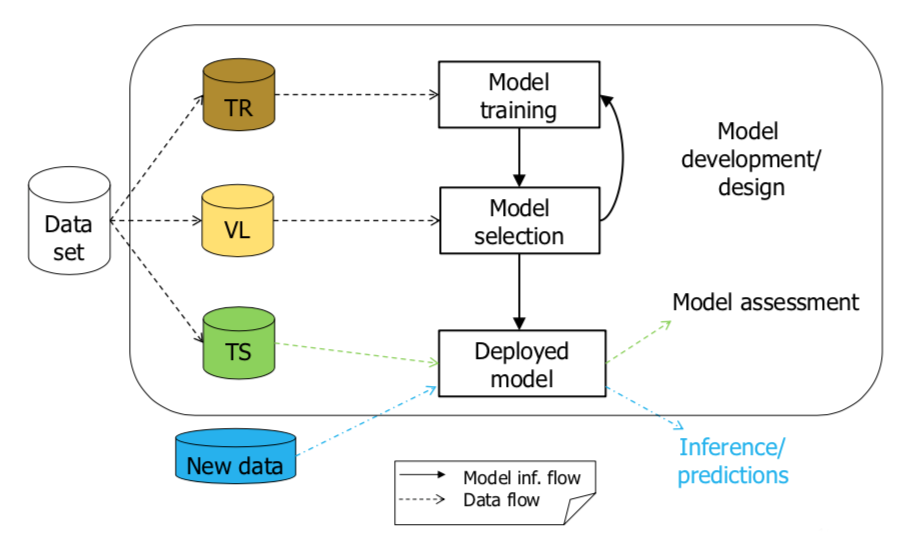
\includegraphics[scale = 0.4]{lectures/1_Introduction/intro_cross_valid_schema.png}
\end{figure}
\begin{center}
    \textbf{Gold rule}:\textit{ Keep separation between goals and use separate data sets}
\end{center}
\subsubsection{Counterexample}
Suppose we have:
\begin{itemize}
    \item 20-30 examples, 1000 random value input variables,
    \item random target 0/1
    \item We select 1 model with 1 input that guess (for chance) 99\% on any tr and vl and ts set splitting (made after initial selection).
\end{itemize}
\begin{center}
Perfect result (a model with accuracy 99\% )? What is wrong? 99\% is not good estimation of the test error (the right one is 50\%).\\

Example:
\begin{tabular}{ |c||c|c|c|c|c|c| } 
 \hline
 $\#$  &      & 25 &26 & 27& &   \\
   \hline\hline
 1 &\dots & 1 & 1 & 1 & \dots & 1 \\ 
 2 &\dots & 0 & 0 & 0 & \dots & 0 \\ 
 3 &\dots & 1 & 1 & 1 & \dots & 1 \\ 
 4 &\dots & 0 & 0 & 0 & \dots & 0 \\ 
 5 &\dots & 0 & 0 & 0 & \dots & 0 \\ 
  \hline\hline
 6 &\dots & 1 & 0 & 1 & \dots & 1 \\ 
 7 &\dots & 1 & 0 & 0 & \dots & 1 \\ 
 \hline
\end{tabular}
\end{center}
Training set is composed by Rows 1-5 and validation set by 6-7. If we choose the feature that share all the same value with the target column (25) we will get 100 of accuracy, but this is not true. So:
\begin{enumerate}
    \item Estimation of error on TR and VL is NOT good risk estimation.
    \item Using the entire dataset for feature/model selection prejudice the
estimation (biased estimation, called subset selection bias ). Test set was implicitly used at the beginning. Test set must be separated in advance, before making any model selection (even of the Feature selection) !
\end{enumerate}


\subsection{Cross-Validation}
Generically we have used the term “cross validation” for:
\begin{itemize}
    \item An approach to model selection based on direct estimation of prediction error by resampling (instead of analytical). \textbf{Choose hyperparmetrs estimating errors}.
    
    \item More specifically for implementations of estimation methods with resampling specifing how to divide data for both model selection and assessment. How to make partitions of the data set : e.g by K-fold CV.
\end{itemize}
\subsubsection{Hold out}
If we are in a data-rich situation, the best approach for both problems is to randomly divide the dataset into three parts: a training set, a validation set, and a test set. 
\begin{figure}[H]
    \centering
    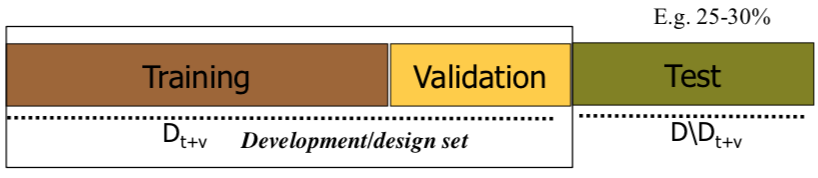
\includegraphics[scale = 0.4]{lectures/1_Introduction/intro_cross_valid.png}
    \caption{Caption}
    \label{fig:5_cross_valid}
\end{figure}
It is difficult to give a general rule on how to choose the number of observations in each of the three parts, as this depends on the signal-to-noise ratio (of the underlying
function) in the data and the training sample size. A typical split might be 50\% for training, and 25\% each for validation and testing.\\

\subsubsection{Hold out and K-fold cross validation}

\begin{figure}[H]
      \centering
      \begin{adjustbox}{minipage=\linewidth,scale=0.7}
      \subfloat[k mutually exclusive subsets]{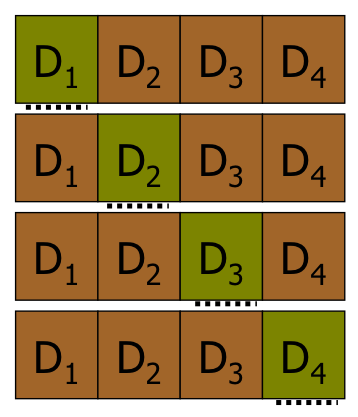
\includegraphics[width=0.45\textwidth]{lectures/1_Introduction/1_kfold.png}\label{fig:5_kfold}}
      \hfill
      \subfloat[mean and standard deviation]{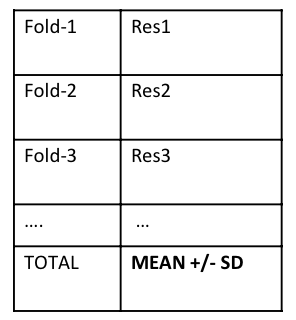
\includegraphics[width=0.45\textwidth]{lectures/5_validation/5_kfold_mean_var.png}\label{fig:5_kfold_mean_var}}
      \caption{k-fold cross validation}
      \end{adjustbox}
\end{figure}
When we have a small number of data, Hold out Cross Validation can make insufficient use of data. To solve this problem we can use another technique called: \textbf{K-fold Cross-Validation}:

\begin{itemize}
    \item Split the data set $D$ into k mutually exclusive subsets $D_1,D_2,\dots,D_k$
    \item Train the learning algorithm on $\frac{D}{D_{i}}$ and test it on $D_i$ repeat this phase k time and then we take the mean of the validation results.
    \item Can be applied for both VL or TS splitting
    \item It uses all the data for training and validation/testing
\end{itemize}

But this technique has some issues: 
\begin{itemize}
    \item How many folds? 3-fold, 5-fold , 10-fold, ...., leave-one-out (when k = n)
    \item Often computationally very expensive (we have to perform training and validation phases k times)
\end{itemize}

Combinable with validation set, double-K-fold CV, ....\\

\noindent\textbf{How many K?}\\
It is interesting to wonder about what quantity K-fold cross-validation estimates. With K = N (Leave-one-out), the cross-validation estimator is approximately unbiased for the true (expected) prediction er- ror, but can have high variance because the N “training sets” are so similar to one another. The computational burden is also considerable, requiring N applications of the learning method. On the other hand, with K = 5  cross-validation has lower variance, we might guess that it estimates the expected error Err, since the training sets in each fold are quite different from the original training set.\\

5 or 10-fold CV are recommended as a good compromise (among bias and variance of estimation) with respect to Leave-one-out cross-validation (LOOCV) (Hastie et al. and
the references therein)

\subsection{An example of model selection and assessment}
\begin{itemize}
    \item Split data in TR and Test set (here simple hold-out or a K-fold CV)

    \item \textit{[Model selection]} Use K-fold CV (internal) over set, obtaining TR e VL set in each folder, to find best hyper-parameters of your model (e.g. polynomial order, lambda of ridge regression, number units in a NN ...): Grid-search with many possible values of the hyper-parameters. For example a k-fold-CV for $\lambda = 0.1$, a CV for $\lambda =0.01$ , ... and then take the best $\lambda$ (by the mean over the validation sets for each fold)
    
    \item Train on the whole TR set the final model
    
    \item \textit{[Model assessment]} Evaluate it on the external test set
\end{itemize}

\subsubsection{Lucky/Unlucky sampling}
Can we avoid to be sensible to the particular partitioning of examples? (bias of the particular sample)
\begin{itemize}
    \item Stratification procedure: stratification is the process of grouping members of the population into relatively
    
    \item Classification: for each (random) partition (TR and TS in hold-out/CV) each class is represented in approximately the same proportions as in the full data set
    
    \item Folder composition: check if order in data related to specific meaning
    
    \item Repeated hold-out method or CV: repeat splitting with different random sampling
    \begin{itemize}
        \item E.g. repeat the CV 10 times an average the results to yield an overall estimation
        \item Useful Especially for comparing different models !
    \end{itemize}
homogeneous subgroups before sampling.
\end{itemize}

\subsubsection{Very few data (informal)}
With very few data: difficult to say whether a sample is representative or not ....
\begin{itemize}
    \item Stratification
    \item Avoid (or consider in evaluation):
    \begin{itemize}
        \item Missing classes or features in training data
        \item Special classes of data not sampled in TR or TS (again stratification)
        \item Prior known outliers can affect the mean test results
        \item On the opposite: selection of only “easy” cases
    \end{itemize}
    \item blind test set can be misleading if it is
    \begin{itemize}
        \item From a different distribution
        \item Measured with different scale, different tolerance, etc.
        \item Uncleaned, unpreprocessed, ...
        \item Extrapolation (out of range data)
    \end{itemize}
\end{itemize}

\subsection{Searching hyperparameters }
Parameters that are not directly learnt within estimators can be set by searching a hyperparameters space (of course by model selection on a validation set).
Search best hyper-parameter values, two approach
\begin{itemize}
    \item Exhaustive Grid Search: exhaustively generates candidates from a grid of parameter values.
    \begin{figure}[H]
        \centering
        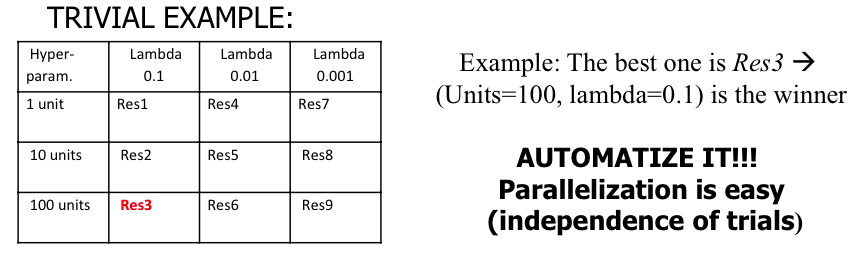
\includegraphics[scale = 0.3]{lectures/5_validation/5_grid_s_1.png}
    \end{figure}
    \item Randomized Parameter Optimization: J.Bergstra,Y.Bengio,(2012). "Random Search for Hyper-Parameter Optimization" J. Machine Learning Research 13: 281–305
\end{itemize}
\noindent\textbf{Grid Search}:\\
The cost of search can be high: Cartesian product between the sets of values for each hyperparameter.
\begin{figure}[H]
    \centering
    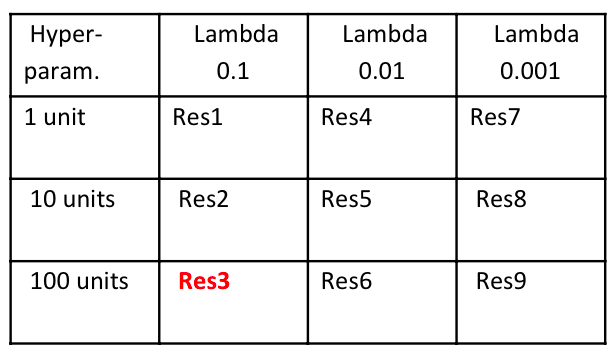
\includegraphics[scale = 0.2]{lectures/5_validation/5_grid_s_2.png}
\end{figure}
$$\#(\text{values in the range})^{\#\text{hyperparameters}}$$
For example $3*3=3^2=9$, What with 5-6 hyperparameters, each with 10 possible different values? we will have a very big number of model to find and evaluate.\\

Can be useful to fix some hyperparameters values in a preliminary experimental phase (since they show to be not relevant)\\

Two (or more) levels of grid search:

\begin{itemize}
    \item Apply a first coarse gird search to the (other) hyperparameters with a table on the combinations of all the possible (e.g. growing exponential) values too find good intervals (regions)

    \item Then a finer grid-search can be performed (over smaller interval and
with selected hyperparameters)
\end{itemize}

\subsection{Error Functions for Evaluation}
\begin{figure}[H]
    \centering
    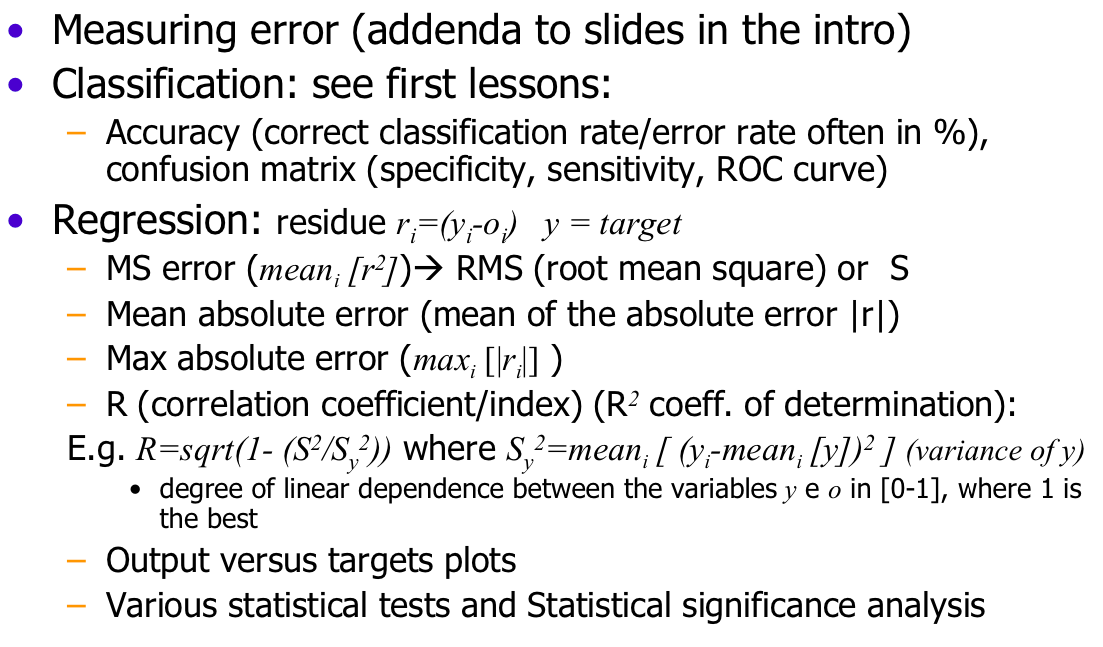
\includegraphics[scale = 0.30]{lectures/5_validation/5_error_function.png}
\end{figure}

\subsection{Bootstrap}
Bootstrap is a random resampling with replacement and repeat it to form different subsets (vd or ts)
\end{document}